\section{Sistemas de Controle}
\label{sec:sistema_controle}
O controle automático é um componente importante e intrínseco em sistemas de veículos espaciais, sistemas robóticos, modernos sistemas de manufatura e quaisquer operações industriais que envolvam o controle de temperatura, pressão, umidade, viscosidade, vazão etc \cite{ogata2011engenharia} [Okata:Eng.Controle Moderno]. Um problema de controle consiste em determinar uma forma de afetar um dado sistema físico de modo que seu comportamento atenda às especificações de desempenho previamente estabelecidas. Como, normalmente, não é possível alterar a estrutura funcional do sistema físico em questão, a satisfação das especificações de desempenho é atingida mediante o projeto e implementação de controladores (compensadores) [apostilha]. Algumas \textbf{definições/terminologias} comuns no contexto de sistema de controle são apresentadas a seguir.

%[Okata:Eng.Controle Moderno]
Segundo \cite{ogata2011engenharia}.
\textbf{Sinal de controle ou variável manipulada.} Como o próprio nome indica, é a grandeza controlada/manipulada. É o sinal que é modificado pelo controlador, de modo a afetar a variável que se está controlando. Geralmente o sinal de controle é a saída do sistema (entrada da planta).\\

\textbf{Planta.} Uma planta pode ser um equipamento, parte de um equipamento ou um conjunto que funciona de maneira integrada, com o objetivo de realizar uma determinada tarefa. Pode ser qualquer mecanismo/objetivo físico a ser controlado (como por exemplo, um motor, um reator ou qualquer componente mecânico no geral).

\textbf{Processos.} Caracteriza-se por ser qualquer operação com um desenvolvimento por mudanças graduais e progressivas que se sucedem de forma a conduzir um resultado ou uma determinada finalidade.

\textbf{Sistemas.} É uma combinação de vários componentes que trabalham em conjunto para atingir um determinado objetivo. O conceito pode ser aplicado tanto para fenômenos físicos quanto para fenômenos abstratos.

\textbf{Distúrbios.} É uma interferência (sinal adverso) que influência na saída de um sistema. Pode ocorrer internamente ao sistema quando externamente.


\textbf{Controle.} Ação por meio da qual se manipula um sistema físico visando fazer com que este atenda um determinado conjunto de especificações determinadas a priori.

\textbf{Controlador.} Dispositivo utilizado para realizar o controle de um sistema físico.



\textbf{Sistema de controle em malha aberta (\emph{Feedforward}).} Sistema de controle que não possui a entrada influenciada pela saída do sistema. Isso quer dizer que, o sinal de saída não é medido nem realimentado para comparação com a entrada (Ver Figura \ref{fig:ilustracao_sistema_malha_aberta}). Devido a natureza desse tipo de controle, a entrada de referência é mapeada para uma saída fixa do controlador. Dessa maneira, a precisão do sistema depende de uma calibração para melhor ajustar/mapear a referência em um determinado sinal de controle.

\begin{figure}[H]
    \centering
    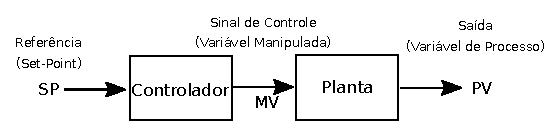
\includegraphics[width=0.8\textwidth]{figuras/ilustracoes/diagrama_sistema_malha_aberta.eps}
    \caption{Diagrama de exemplificação de sistema de controle em malha aberta.}
    \label{fig:ilustracao_sistema_malha_aberta}
\end{figure}

\textbf{Sistema de controle em malha fechada.} Difere essencialmente do em malha aberta, pois neste tipo a entrada do controlador é influenciada pela saída da planta (variável de processo) (Ver Figura \ref{fig:ilustracao_sistema_malha_fechada}). Esse tipo de sistema de controle também é denominado de controle com realimentação (controle com \emph{Feedback}). A relação entre a saída e a entrada de referência se dar por meio da comparação entre elas, utilizando a diferença como meio de controle.

\begin{figure}[H]
    \centering
    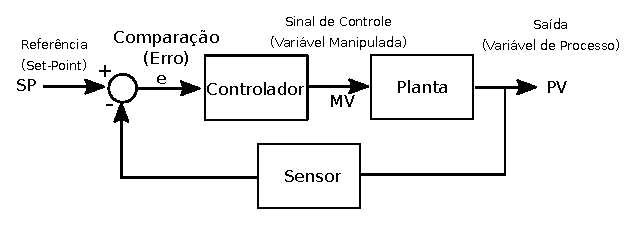
\includegraphics[width=0.8\textwidth]{figuras/ilustracoes/diagrama_sistema_malha_fechada.eps}
    \caption{Diagrama de exemplificação de sistema de controle em malha fechada.}
    \label{fig:ilustracao_sistema_malha_fechada}
\end{figure}


Segundo [Okata] as principais vantagens do sistema de controle em malha aberta são:
\begin{enumerate}
    \item São de fácil construção/implementação e fácil manutenção.
    \item Não apresentam problemas de estabilidade.
    \item São mais adequados em situações em que a medição precisa da saída é um problema.
\end{enumerate}

E algumas desvantagens:

\begin{enumerate}
    \item Distúrbios e mudanças na calibração causam erros, e a saída pode apresentar diferenças
    em relação ao padrão desejado.
    \item Para que a saída mantenha a qualidade requerida, é necessária uma regulagem periódica.
\end{enumerate}


\subsection{Controlador PID}
% Controlador PID
% Controlador malha aberta Feedforward
Um controlador clássico do tipo \emph{Feedback} e que ainda é muito utilizado é o controlador proporcional Integral derivativo (PID). Como o próprio nome indica, esse tipo de controlador une as ações derivativa, integral e proporcional. A ação proporcional faz com que o erro diminua e influência no tempo de resposta do sistema, a ação integral elimina o erro de regime e a ação derivativa influência no tempo de resposta do sistema, por meio da antecipação do erro.

Definindo-se os seguintes sinais no tempo: $u(t)$ como sinal de saída (sinal de controle) e $e(t)$ como o erro entre a referência e o valor atual da saída da planta, o controlador pode ser definido como:

\begin{equation}
    u(t) = K_{p}e(t) + K_{i} \int^{t}_{0}e(\tau)d\tau + K_{d}\frac{d e(t)}{dt}
\end{equation}

Aplicando a transformada \emph{Laplace} temos,

\begin{equation}
    \frac{U(s)}{E(s)} = K_{p} + \frac{K_{i}}{s} + K_{d}s
\end{equation}

Sendo,

\begin{itemize}
    \item $K_p$: O ganho proporcional.
    \item $K_i$: Ganho integral.
    \item $K_d$: Ganho derivativo.
    \item $s$: Frequência complexa.
\end{itemize}

Esse tipo de controlador pode ser utilizado em mais três formas básicas além do padrão PID: Controle Proporcional (P). Apenas a ação proporcional; Controle Proporcional Integral (PI) e Controle Proporcional Derivativo (PD).

\begin{figure}[H]
    \centering
    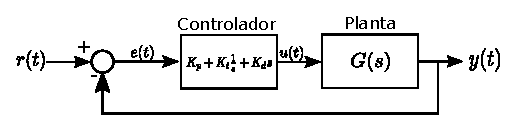
\includegraphics[width=\textwidth]{figuras/ilustracoes/diagrama_controlador_PID.eps}
    \caption{Diagrama de um sistema controlado por PID.}
    \label{fig:diagrama_controlador_PID}
\end{figure}

A Figura \ref{fig:diagrama_controlador_PID} ilustra em diagrama de blocos o uso do controlador PID. Onde $r(t)$ é o sinal de referência (\emph{set-point}), $y(t)$ é a saída da planta e $G(s) = Y(s)/U(s)$ é a função de transferência da panta.

\subsection{Sistemas de Primeira Ordem}

Um sistema de primeira ordem apresenta a seguinte forma genérica:

\begin{equation}
    T\dot{y} + y = Ku
\end{equation}

E em \emph{Laplace} com a seguinte função de transferência,

\begin{equation}
    G(s) = \frac{K}{Ts + 1}
\end{equation}

E sua resposta no tempo para uma entrada do tipo degrau unitário ($u(t) = 1 \xrightarrow{\mathscr{L}} U(s) = 1/s$),

\begin{equation}
    y(t) = K \left(1 - e^{-t/T} \right)
\end{equation}

Sendo $K$ o ganho do sistema e a constante $T$ é conhecida como constante de tempo do sistema e $T > 0$. A Figura \ref{fig:saida_sistema_primeira_ordem_no_tempo} ilustra o comportamento no tempo de um sistema de primeira ordem e a influência da constante de tempo $T$ na resposta do sistema.

\begin{figure}[H]
    \centering
    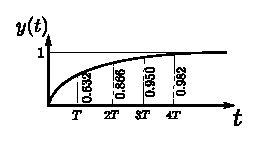
\includegraphics[width=0.7\textwidth]{figuras/ilustracoes/resposta_no_tempo_sistema_primeira_ordem.eps}
    \caption{Resposta no tempo ao degrau unitário de um sistema de primeira ordem com ganho unitário e contante de tempo $T$.}
    \label{fig:saida_sistema_primeira_ordem_no_tempo}
\end{figure}

% O erro de regime é a diferença entre os sinais de entrada e de saída na região de regime da resposta. Ou seja, $t \xrightarrow{} \infty$.